\documentclass[12pt]{article}

\usepackage[colorlinks=true,urlcolor=blue]{hyperref}
\urlstyle{same}

\usepackage{graphicx}
\graphicspath{{./figures/}}

\usepackage{mathptmx}
\usepackage[outdir=./figures/]{epstopdf}
\usepackage{float}
\usepackage[font=footnotesize]{caption}
\usepackage{wrapfig}
%\usepackage[a4paper]{geometry}
\usepackage{microtype}
\usepackage{booktabs}



\author{Gabriel Siqueira Kakizaki}
\date{\today}
\title{\textbf{Road Vehicle Accident Severity Prediction in Seattle, WA}}

\begin{document}

%\pagenumbering{gobble}
\maketitle
%\newpage
%\pagenumbering{arabic}

%\tableofcontents
%\newpage


\section{Introduction}

\subsection{Problem and Background}

Road vehicle accidents are a problem that in 2019 caused more than 38 thousand estimated deaths, and injuries in about 4.4 million people, only in the USA.\spacefactor\sfcode`.{} In this project we will explore the use of machine learning models to predict the accident severity, using open data provided by the city of Seattle.

\subsection{Stakeholder Interest}

Policymakers need information on what factors cause road accidents, especially the severe ones, when creating or improving on existing preventive policies. Data analysis can help extract the needed insights from the data.

\section{Data}

\subsection{Data Sources}

The city of Seattle makes data about road vehicle crashes available, under the Public Domain Dedication and License (PDDL). The most recent dataset can be downloaded from \href{https://data-seattlecitygis.opendata.arcgis.com/datasets/collisions}{here}.

\subsection{Data Description}

Downloaded data had information about approximately 195 thousand road vehicle collisions, from 2004 to May 2020. Examples of some relevant features are latitude and longitude coordinates, date and time of occurrence, weather, road and light conditions, among others.

To prepare the data for analysis and modeling, first we removed the entries missing the location, which represented 2.74\% of the total rows.
Second, we removed columns which missing values represented more than 10\% of the total values, although some of them could have had a good predictive value  (if the driver was speeding, for example).
Third, we imputed the remaining missing values with the most common value for each of the columns. After, we also manually joined categories with low frequency for the weather, road and light conditions into `Other'.

Another problem that we had, common in real world classification projects is the balance of the target variable. In our binary classification problem, approximately 70\% of the cases represented a low severity collision (property damage), while only 30\% were a high severity collision (with injury).

\subsection{Feature Engineering}

We had to transform the data to make it useful input for the models. First we removed redundant columns. In some cases there were two columns for the same information (e.g., a code and a description for the severity of the accident), so we kept only the numeric one.

Second, we converted categorical variables to numeric ones using one hot encoding, except for the date and time of incident. Because time is cyclical (e.g., the first hour of the day is close to the last), we extracted the day of the week in which the accident happened, and used sine-cosine encoding to keep its cyclical nature.

Third, especially because we want the feature's importance from the models, we addressed multicollinearity by further removing redundant information. We also removed the SDOT (Seattle Department of Transportation) collision code and the State collision code as they had many categories, causing encoding to generate high dimensional, sparse data.

\section{Methods}

\subsection{Exploratory Data Analysis (EDA)}

First thing we did was to verify the problem of class imbalance. There were 70\% of low severity accidents and 30\% of high severity accidents. As we got much data, the number of high severity accidents is almost 60 thousand, so we will simply use a random under sampler to balance the classes while making the models.

\subsubsection{Relationship Between Accidents and Date-Time}

For the analysis of accidents in relation to time, the year of 2020 was removed due to incompleteness of the data. The hypothesis is that the quantity is different across some specific time frames. We calculated the total number of accidents per year, month, day of month, day of week and hour.

Regarding total accidents per year, the quantity was higher around 2006 and 2015, but otherwise was stable around 10 thousand.

There wasn't a significant difference between months. The month with less total accidents was February, but it also is the month with the least number of days, so we have to be careful with this information. The month with the most number of accidents was October.

%\begin{figure}
%        \centering
%        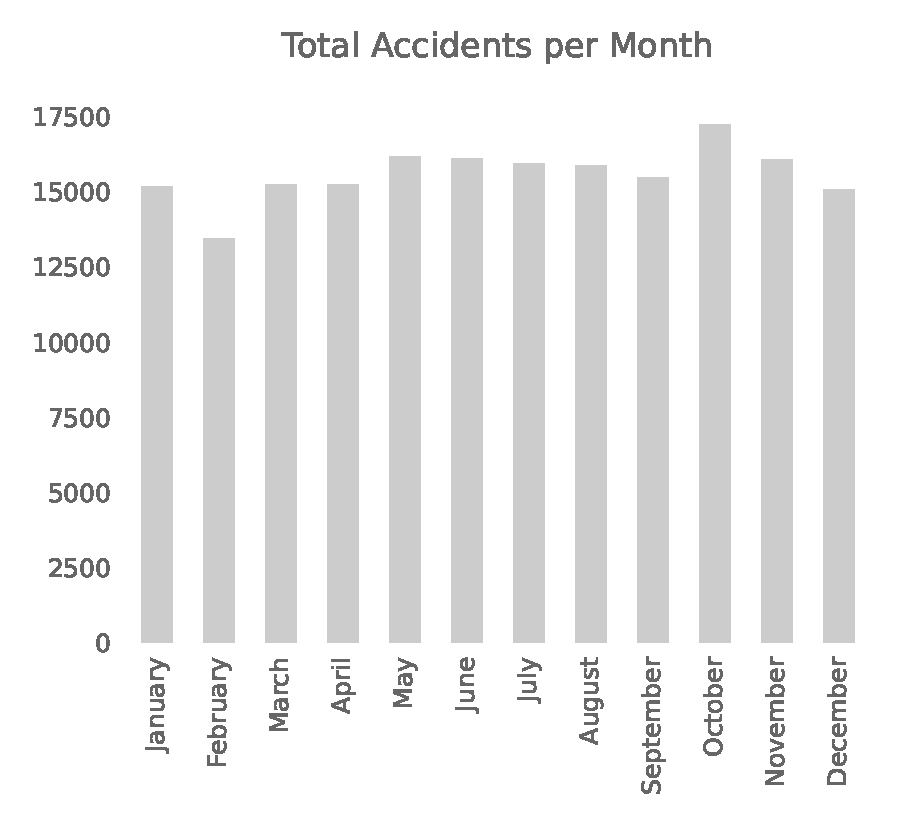
\includegraphics[width=0.7\textwidth]{plot_months.eps}
%        \caption{Total accidents for 2004-2019 per month.\label{fig:months}}
%\end{figure}

The day of month also had little or no influence on the number of accidents. The 31st day of the month also seemed to have fewer total accidents, but like the problem with February, only seven out of the twelve months have 31 days.

The day of the week was the most useful for us to input in the models. Friday had the highest number of accidents, while Sunday had the lowest, with the difference being around 10 thousand, as shown in \autoref{fig:day_of_week}. This could possibly be because there is more traffic and more people on the streets on Friday than on Sunday.

\begin{figure}
        \centering
        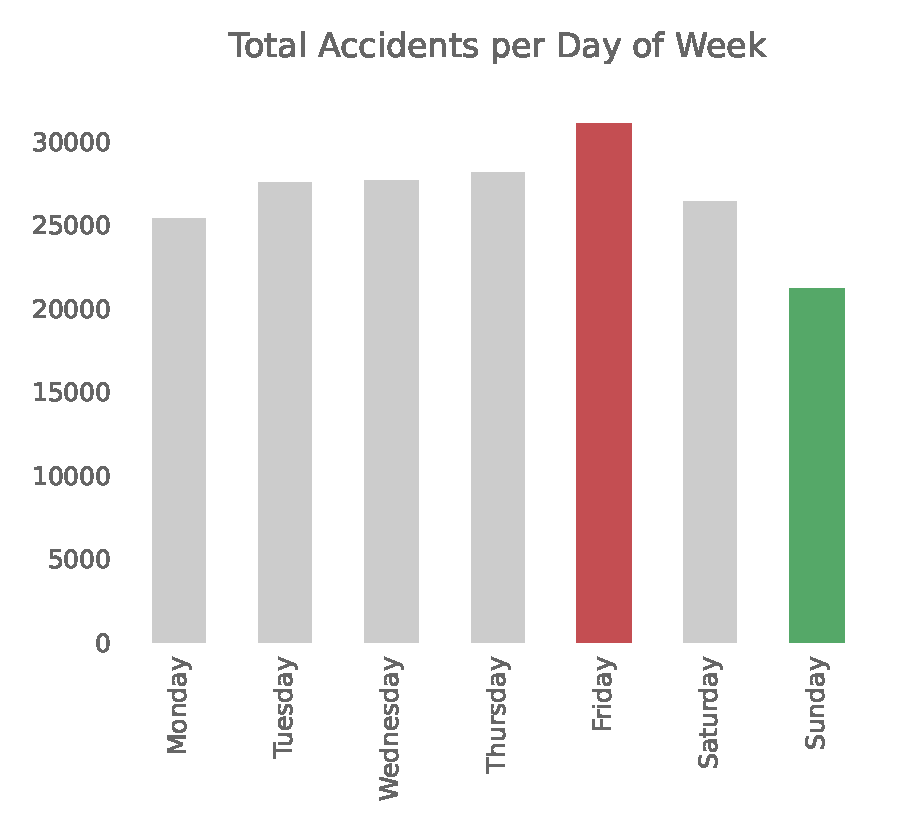
\includegraphics[width=0.7\textwidth]{plot_day_of_week.eps}
        \caption{Total accidents for 2004-2019 per day of week.\label{fig:day_of_week}}
\end{figure}

The hour of the day also had an impact on the number of accidents. One problem is that the number is the highest at midnight, very much likely because of missing values, so we couldn’t use this information as input to our machine learning models. But ignoring the accidents happening at midnight, as we can see in \autoref{fig:hour}, the number of accidents is higher at peak hours, and the highest at 5 pm, then it lowers as there is less movement in the streets, reaching the lowest at 4 am.

\begin{figure}
        \centering
        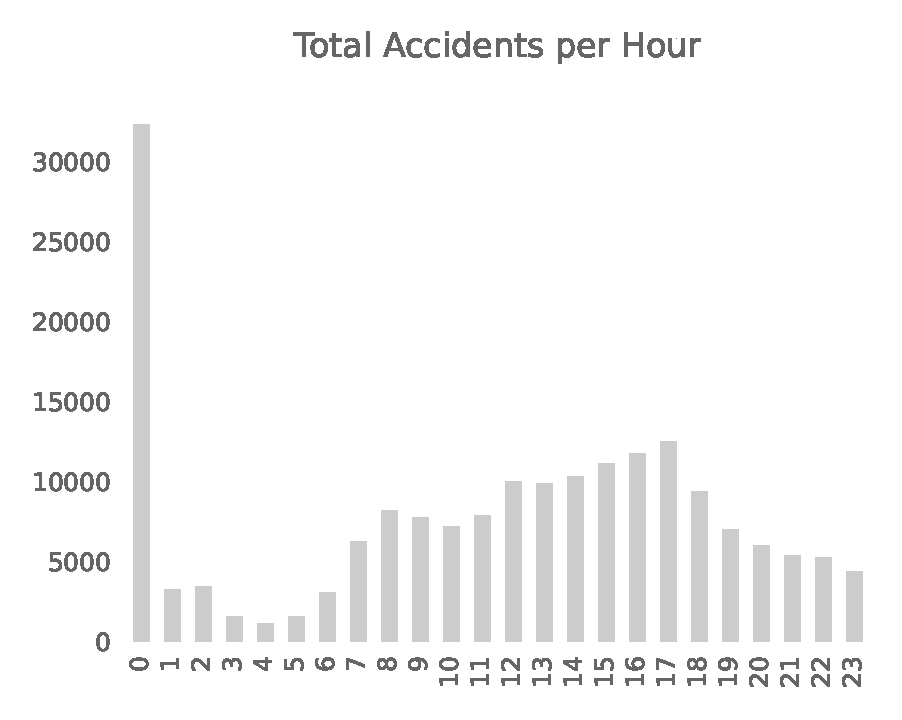
\includegraphics[width=0.7\textwidth]{plot_hour.eps}
        \caption{Total accidents for 2004-2019 per hour.\label{fig:hour}}
\end{figure}

\subsubsection{Categorical Variables}

We used cross tabulation and bar plots to visualize the relation between the accident severity and the other categorical variables. As our variable of interest is imbalanced, if a category don't have any impact on the severity we should see 70\% of low severity and 30\% of high severity, rather than a 50-50\% split.

First, we analyzed variables with only two categories. The address type was divided into block and intersection. Blocks had 6\% less severe accidents when comparing with the total, while intersections had 13\% more, as shown in \autoref{fig:addrtype}.
\begin{figure}
        \centering
        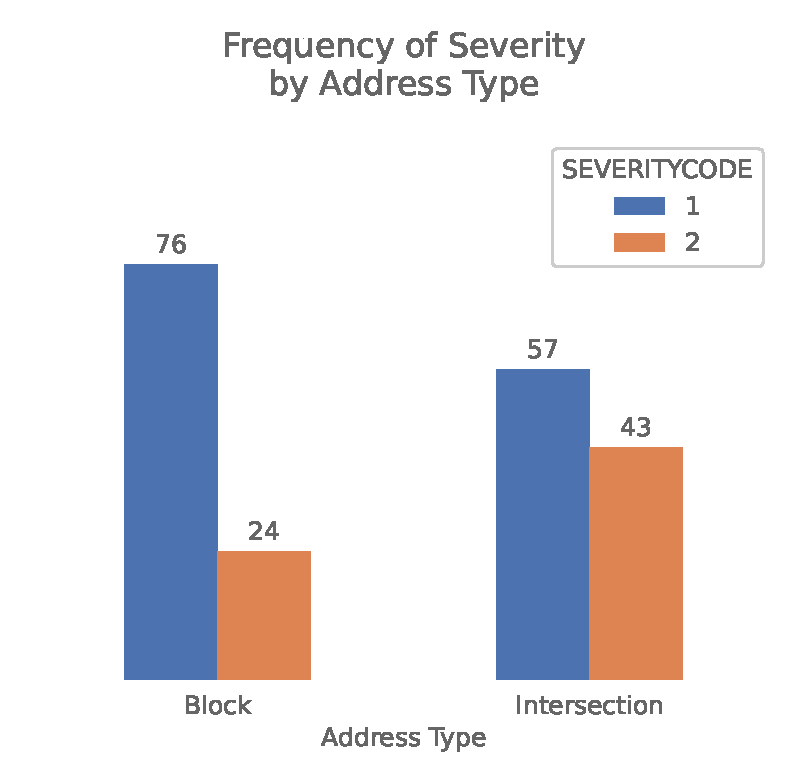
\includegraphics[width=0.7\textwidth]{plot_addrtype.eps}
        \caption{Accidents severity frequency by address type.\label{fig:addrtype}}
\end{figure}
The other two variables contained yes or no values. If the driver was not under influence of drugs or alcohol, the ratio of accidents remained the same, but if the driver was under influence, we saw a 9\% increase in the quantity of severe accidents. On the other hand, if the driver hit a parked car, 94\% of the time was a collision without injury.

Second, we analyzed variables with multiple categories. Weather and road conditions are related to each other. In raining and wet road conditions we saw an increase in severe accidents, in clear weather and dry road the ratio was the same and in snowing weather and ice/snow/slush road we saw a decrease in severe accidents.

Collision type also had useful information. In \autoref{fig:collisiontype}, we could see that the highest ratios of injury collisions were when a car hit a pedestrian or a bicycle. Head on, rear ended, left turn and angles collision types were also more dangerous than right turn and sideswipe. The least severe collision type is with a parked car.
\begin{figure}
        \centering
        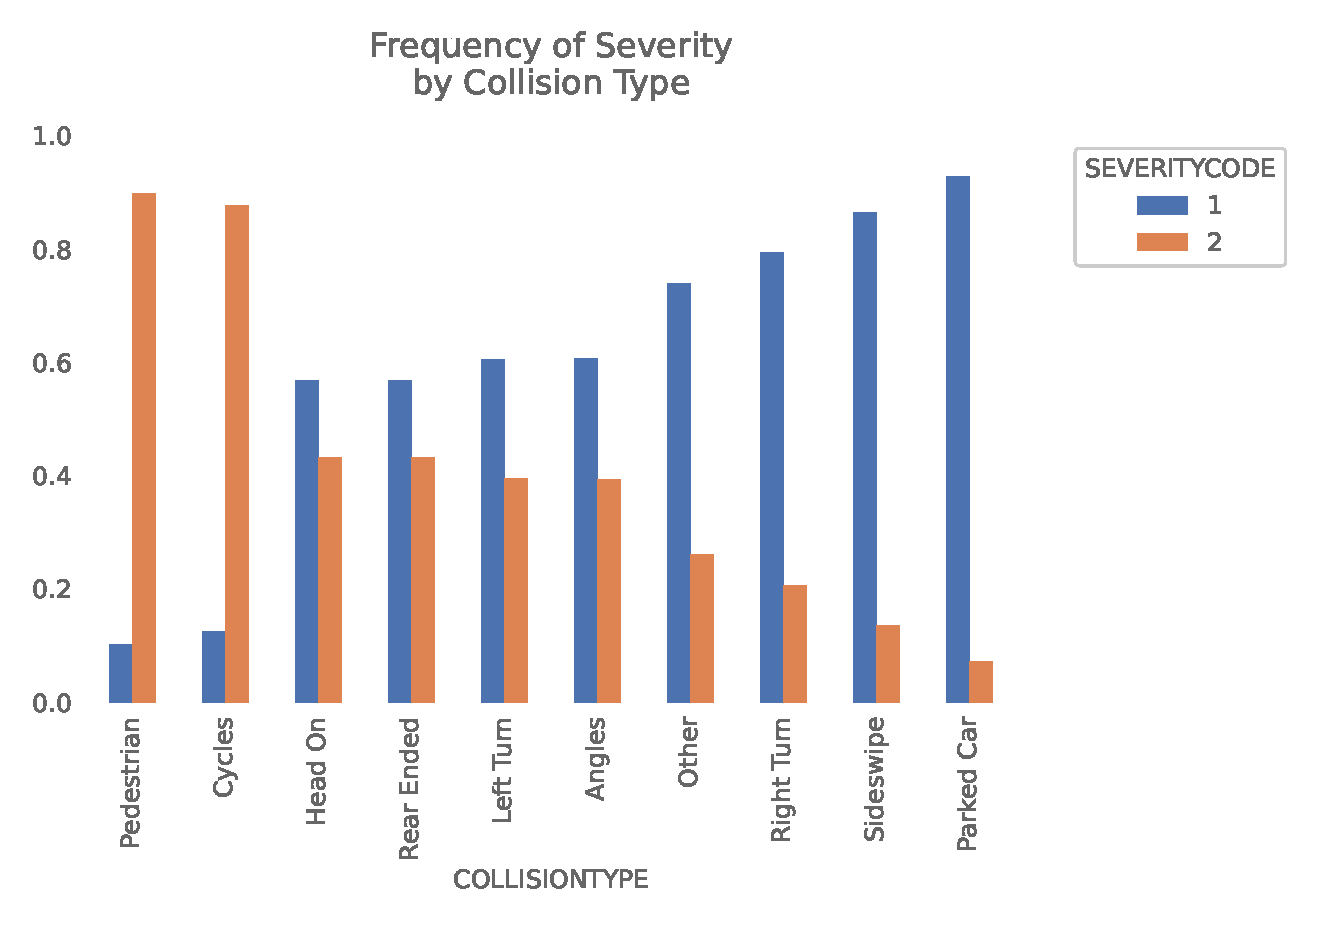
\includegraphics[width=0.9\textwidth]{plot_collisiontype.eps}
        \caption{Accidents severity frequency by collision type, sorted by high severity.\label{fig:collisiontype}}
\end{figure}

\subsection{Modeling}

After the features were selected, we choose to use a stratified split on our data due to the class imbalance, with 20\% for training and 80\% for testing. The models chosen for prediction were Logistic Regression, to serve as a baseline to compare with Random Forests and Extreme Gradient Boosting, that were chosen because they don’t have the same prior assumptions as Logistic Regression (e.g., the features are linearly related).

For every algorithm, two different models were made. The first one was trained on the imbalanced training set. For the second one, we used the random under sampling technique with cross validation and parameter tuning using grid search on the training set. This process is automatically handled by the imbalanced-learn library pipeline, and has the advantage of being possible to train the models on balanced datasets with cross validation without data leakage.

For evaluation, we used the following methods and metrics: precision, recall, f1-score, area under the curve (AUC) and confusion matrix. We also calculated SHAP Values to get the feature importances for the XGBoost model. All models were evaluated using the test set.

\section{Results}

All algorithms had similar performance. As shown in \autoref{tab:metrics}, imbalanced models had a better recall on average because it was better for the low severity accidents, but worse for high severity ones. Balanced models were better when predicting high severity by having a higher recall and f1-score on this class.

\begin{table}[h]
        \centering
        \begin{tabular}[c]{ c c c c c }
                \toprule
                Imbalanced Models & Precision & Recall & F1-score & AUC \\
                \midrule
                Logistic Regression & 0.75 & 0.75 & 0.71 & 0.79\\
                Random Forest & 0.73 & 0.75 & 0.72 & 0.77 \\
                XGBoost & 0.75 & 0.76 & 0.72 & 0.79 \\
                \midrule
                Balanced Models \\
                \midrule
                Logistic Regression & 0.75 & 0.67 & 0.68 & 0.79 \\
                Random Forest & 0.76 & 0.67 & 0.69 & 0.79 \\
                XGBoost & 0.76 & 0.67 & 0.68 & 0.79 \\
                \bottomrule
        \end{tabular}
        \caption{Weighted average precision, recall, f1-score and AUC for the models.\label{tab:metrics}}
\end{table}

In \autoref{fig:xgbmatrix}, we can see the normalized confusion matrix for the balanced XGBoost model, and in \autoref{fig:xgbroc}, we can see its ROC curve.

We used the SHAP feature importance to explain predictions generated by the XGBoost model. In \autoref{fig:xgbshapbar}, it is easier to visualize the amount of the impact each feature had on the predictions, and in \autoref{fig:xgbshapbee}, we can also see how the values of the features increase or decrease predicted accident severity.

\begin{figure}
        \centering
        \includegraphics[width=0.6\textwidth]{plot_xgb_confmatrix.eps}
        \caption{XGBoost confusion matrix, normalized across rows.\label{fig:xgbmatrix}}
\end{figure}

\begin{figure}
        \centering
        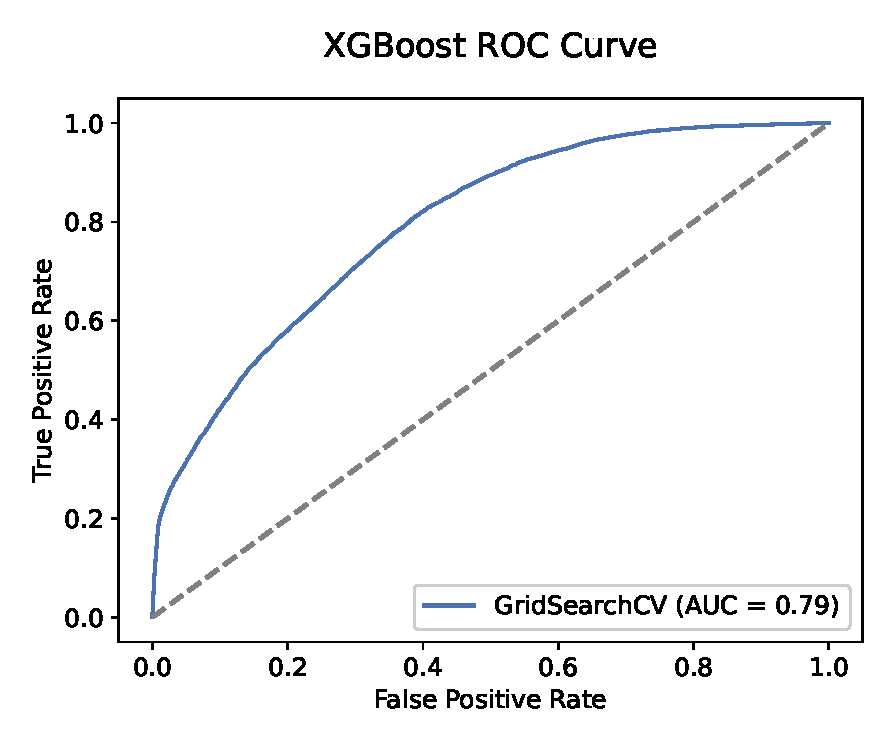
\includegraphics[width=0.6\textwidth]{plot_xgb_roc.eps}
        \caption{XGBoost ROC curve.\label{fig:xgbroc}}
\end{figure}

\begin{figure}
        \centering
        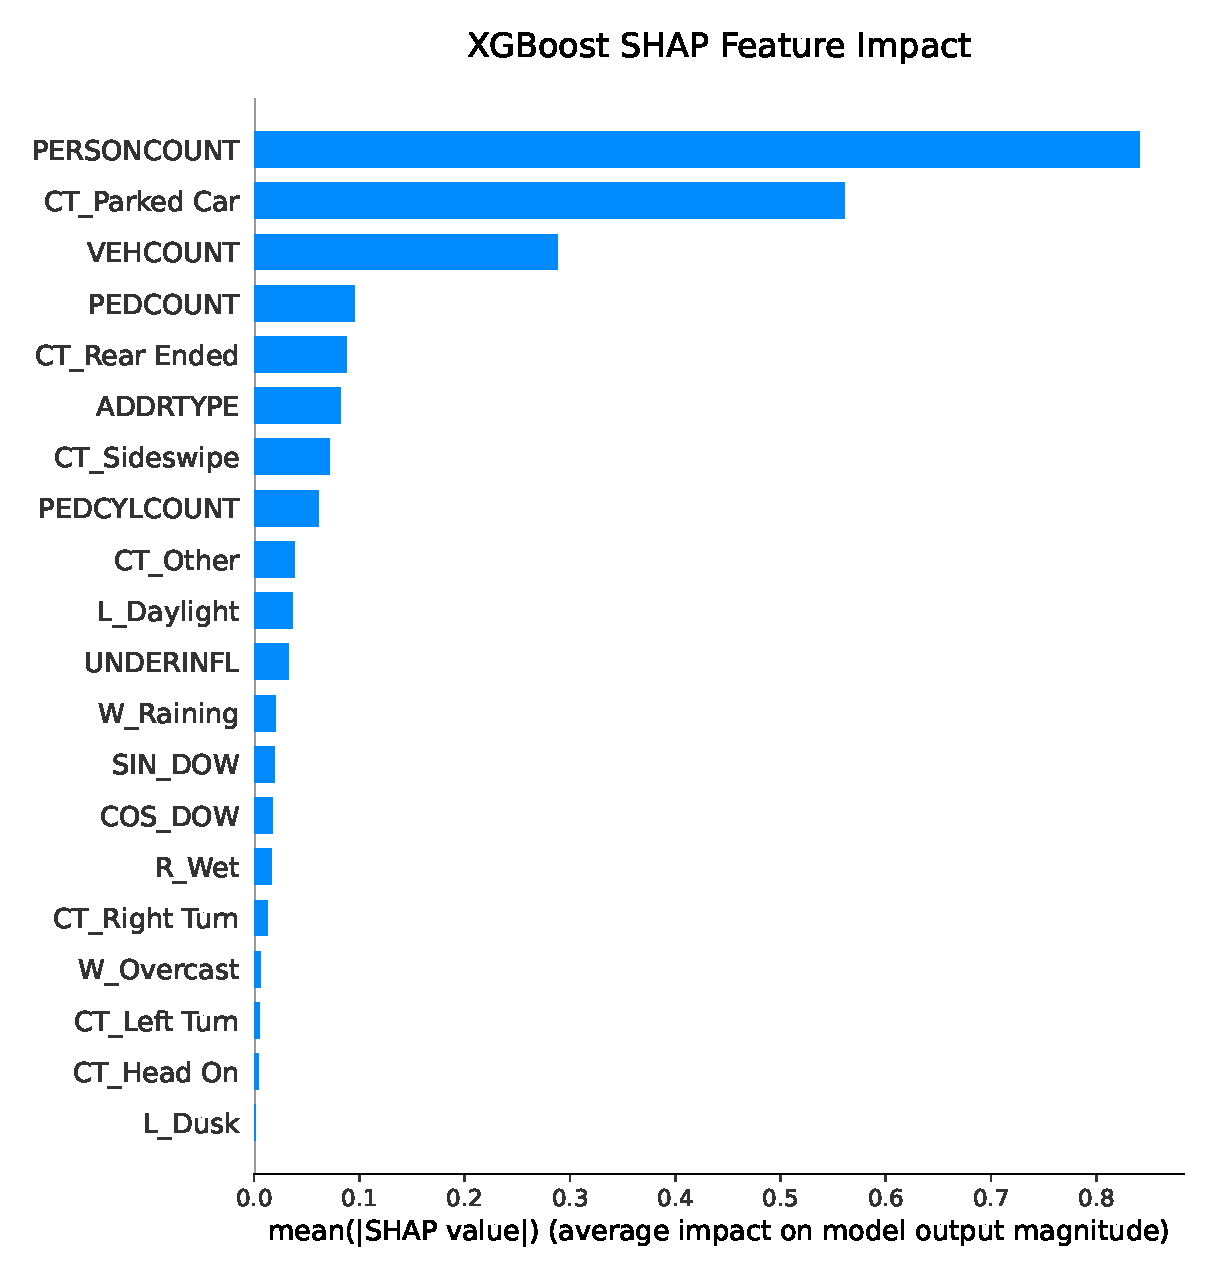
\includegraphics[width=\textwidth]{plot_shap_bar.eps}
        \caption{XGBoost SHAP bar plot.\label{fig:xgbshapbar}}
\end{figure}

\begin{figure}
        \centering
        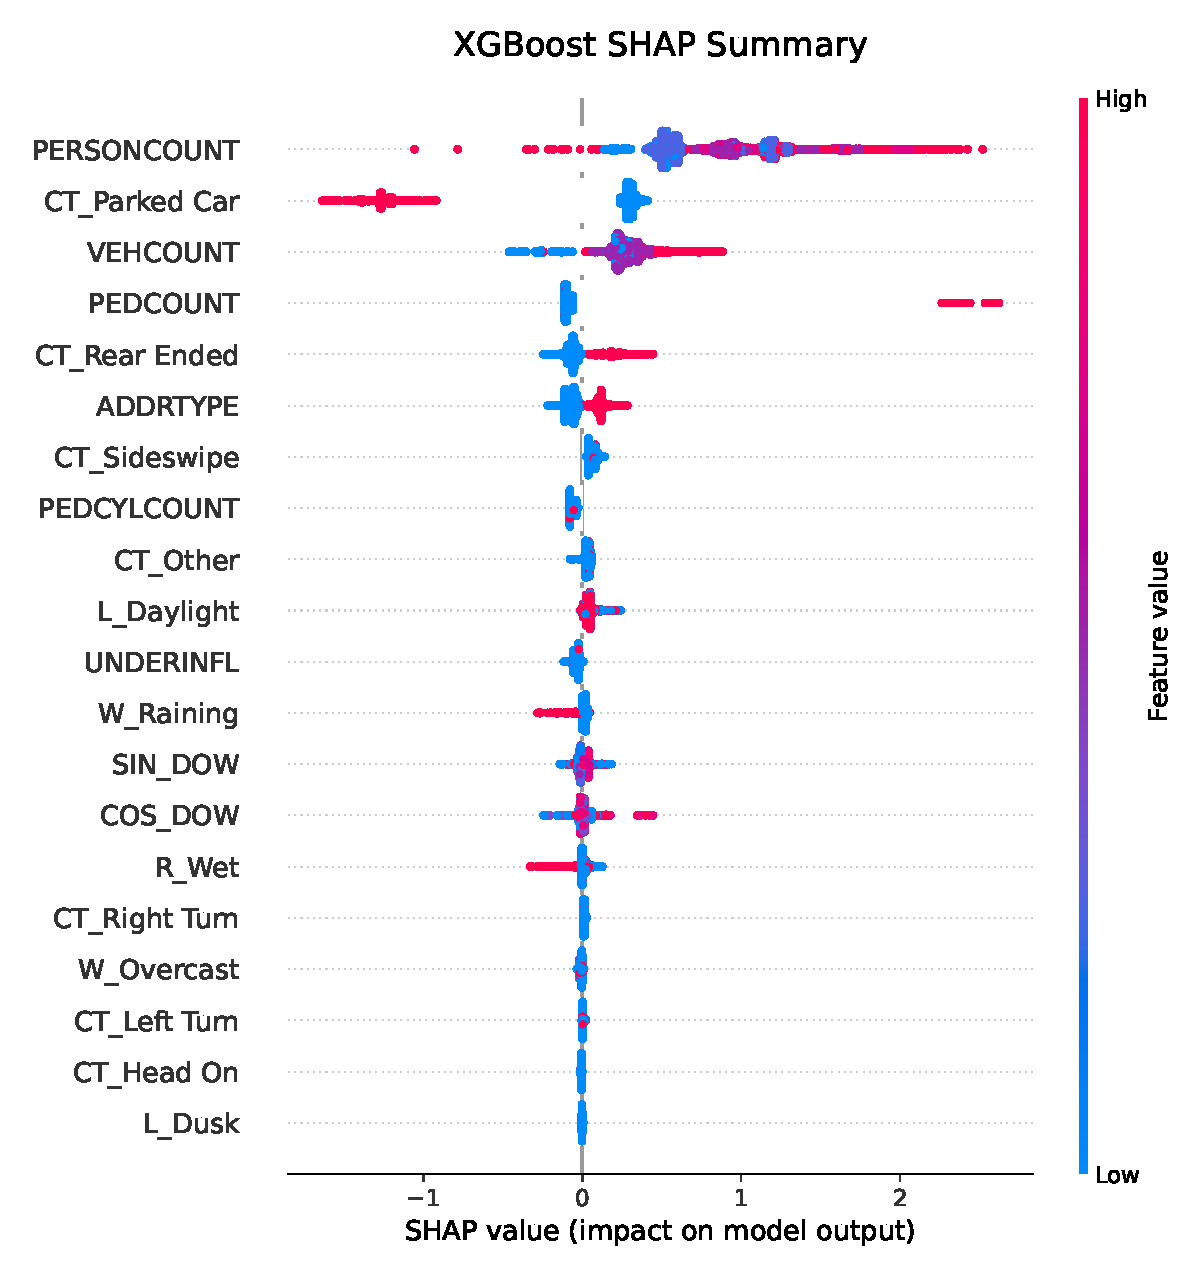
\includegraphics[width=\textwidth]{plot_shap_beeswarm.eps}
        \caption{XGBoost SHAP beeswarm plot.\label{fig:xgbshapbee}}
\end{figure}

\newpage

The model explanation confirms some of the insights we had on the EDA.\spacefactor\sfcode`.{} The most important feature was the number of people involved in the accident. The second one was if the crash was into a parked car. As we saw in \autoref{fig:collisiontype}, most of the crashes into parked cars are of low severity, and on the other hand, most accidents involving pedestrians are of high severity. Our features sine and cosine day of week were also useful for the models.

\section{Discussion}

Predicting road vehicle accident severity with open data is feasible. Feature engineering is a critical step in this process, that will have a big impact on the performance of the models and in its applicability for future predictions.

\subsection{Limitations}

Although machine learning models are useful in predicting accident severity, in this study they rely only on data collected after the accident, making it difficult to make predictions beforehand. Also, only data about the city of Seattle was used, limiting the model usefulness as data from other cities might be in different formats, or the accident severity conditions might differ.

\subsection{Recommendations}

The use of other kinds of data that can be gathered more easily, such as weather or traffic when the collision happened might improve the model resolution and make it possible to predict accidents some time before or even give an estimate of the risk of collision in real-time.

\section{Conclusion}

In this study we analyzed the road vehicle collisions in the city of Seattle, identifying features that impact the severity of the accident. If it happens at an intersection, involves pedestrians or bicycles, happens to be a head on, rear ended or left turn collision, it is more likely to be severe. Peak hours and more movement on the streets means more accidents. We also built classification models to predict the accident severity based on the available data that were used to explain how the features impact severity, and can also be used to simulate different accident conditions.

\end{document}
